\documentclass[12pt,aspectratio=169]{beamer}

\usepackage{minted}

\usetheme[progressbar=frametitle, numbering=fraction]{metropolis}
\usepackage{appendixnumberbeamer}

\usepackage{booktabs}
\usepackage[scale=2]{ccicons}

\usepackage{pgfplots}
\usepgfplotslibrary{dateplot}

\usepackage{xspace}
\usepackage{tikz}
\newcommand{\themename}{\textbf{\textsc{metropolis}}\xspace}

% Chinese Fonts (Fontset: fandol,ubuntu)
\usepackage{ctex}

% Math Fonts
\usefonttheme{professionalfonts} 
\usepackage{mathspec}
% \setsansfont[BoldFont={Fira Sans},Numbers={OldStyle}]{Fira Sans Light}
% \setmathsfont(Digits)[Numbers={Lining, Proportional}]{Fira Sans Light}

% Change Color of the theme
\usepackage{xcolor}
\definecolor{DarkGrey}{HTML}{353535}
\definecolor{ECNURed}{RGB}{164,31,53}
\definecolor{ECNUBrown}{RGB}{134,117,77}
\setbeamercolor{normal text}{ fg= DarkGrey  }
\setbeamercolor{alerted text}{ fg= ECNURed  }
\setbeamercolor{example text}{ fg= ECNUBrown  }

% Bolder Fonts for presenting in a large room 
\setsansfont[BoldFont={Fira Sans SemiBold}]{Fira Sans Book}

\title{搜索算法}
\subtitle{深度优先与广度优先搜索}
\date{\today}
\author{罗江楠}
\institute{哈尔滨工业大学(威海)}
\titlegraphic{\hfill
\includegraphics[height=1cm]{hitwh.png}}

\begin{document}

\maketitle

\begin{frame}{目录}
  \setbeamertemplate{section in toc}[sections numbered]
  \tableofcontents[hideallsubsections]
\end{frame}

\section[引言]{Introduction}

\begin{frame}[fragile]{引言}
  搜索算法是各种高级算法的基石,比如求解最短路径问题,求解最小生成树问题,求解最大流问题等。

  搜索算法的大致分为两种,分别为深度优先搜索算法(Depth First Search, DFS)和广度优先搜索算法(Breadth First Search, BFS)。

  \begin{figure}
    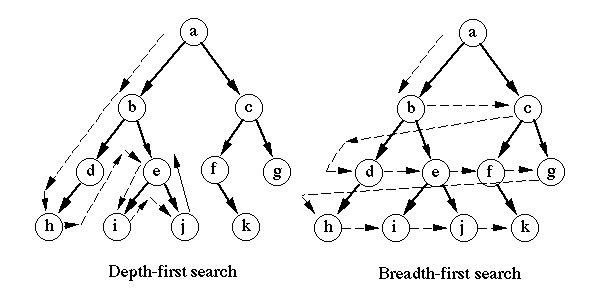
\includegraphics[height=100pt]{dfsbfs.png}
  \end{figure}
\end{frame}

\section[深度优先搜索]{Depth First Search}

\begin{frame}[fragile]{深度优先搜索}
  \begin{itemize}
    \item 尽可能深地搜索树的分支
    \item 直到所有可能情况都被完全搜索一遍
  \end{itemize}
\end{frame}

\begin{frame}[fragile]{例题:整数分解}
  \begin{itemize}
    \item 求解有多少种将正整数 $n$ 分解为 $3$ 个正整数相加的方案
    \item 两种分解方案不同当且仅当加数中的其中一个数字不相同
    \item 例如 $4=1+1+2=1+2+1=2+1+1$ 共有 $3$ 种不同的分解方式
  \end{itemize}
\end{frame}

\begin{frame}[fragile]{例题:整数分解}
  考虑你们之前学过的枚举算法
  \begin{minted}{cpp}
for (int i = 1; i <= n; ++ i)
  for (int j = 1; j <= n; ++ j)
    for (int k = 1; k <= n; ++ k)
      if (i + j + k == n)
        printf("%d = %d + %d + %d\n", n, i, j, k);
  \end{minted}
  \pause
  时间复杂度 $O(n^3)$
\end{frame}

\begin{frame}[fragile]{例题:整数分解}
  可以考虑优化枚举的上下界,可以将复杂度降低到 $O(n^2)$
  \begin{minted}{cpp}
for (int i = 1; i <= n - 2; ++ i)
  for (int j = 1; j <= n - i - 1; ++ j)
    printf("%d = %d + %d + %d\n", n, i, j, n - i - j);
  \end{minted}
\end{frame}

\begin{frame}[fragile]{例题:整数分解}
  \begin{itemize}
    \item 但是如果将题目改成分解成 $4$ 个正整数的和呢?\pause
    \item 写 $4$ 重 \verb|for| 循环?\pause
    \item 如果改成 $m$ 个正整数呢?\pause
    \item 写 $m$ 重 \verb|for| 循环?\pause
    \item 此时就需要运用这个被称为\textbf{深度优先搜索}的算法了
  \end{itemize}
\end{frame}

\begin{frame}[fragile]{深度优先搜索算法}
  深度优先搜索算法一般使用递归的算法,遵从以下流程
  \begin{itemize}
    \item 首先判断搜索的当前状态是否满足\textbf{结束条件}
    \item 如果满足结束条件则输出当前状态并返回
    \item 接下来考虑枚举当前状态的每一个可能的下一个状态的转移
    \item 将该转移应用到当前的状态中
    \item 向下递归搜索
    \item 将当前状态恢复为转移前的状态
  \end{itemize}
\end{frame}

\begin{frame}[fragile]{例题:整数分解}
  \begin{minted}{cpp}
int ans[100]; // 用于储存当前分解方案的数组
void dfs(int x, int k) { // 将 x 分解成 k 个正整数
  if (k == 1) { // 搜索的结束条件
    ans[k] = x; output(ans); // 输出方案
    return;
  }
  for (int i = 1; i <= x - k + 1; ++ i) {
    ans[k] = i; // 记录方案
    dfs(x - i, k - 1); // 递归搜索
  }
}
  \end{minted}
\end{frame}

\begin{frame}[fragile]{例题:整数分解}
  \begin{figure}
    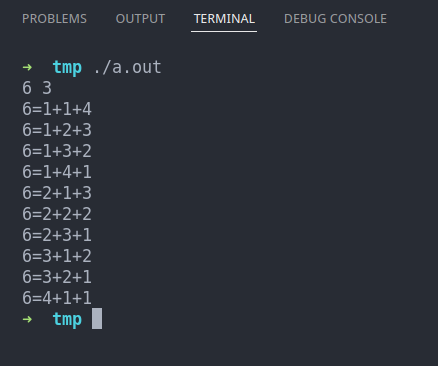
\includegraphics[height=200pt]{example1.png}
  \end{figure}
\end{frame}

\begin{frame}[fragile]{复杂度分析}
  每个答案都只会被枚举到一次,因此算法的时间复杂度与答案规模相同\pause

  $$O({n-1 \choose m-1})$$
\end{frame}

\begin{frame}[fragile]{例题:全排列}
  求 $n$ 个元素的全排列。

  如 $n=3$ 时

  \begin{verbatim}
1 2 3
1 3 2
2 1 3
2 3 1
3 1 2
3 2 1
  \end{verbatim}
\end{frame}


\begin{frame}[fragile]{例题:全排列}
  \begin{minted}{cpp}
int vis[100]; // vis[i] 表示数字 i 是否已经用过
int ans[100]; // 用于保存当前的排列状态
void dfs(int depth) { // 参数 depth 表示当前递归的深度
  if (depth == n + 1) { // 如果所有数字都选完了
    output(ans); return; // 输出并返回
  }
  for (int i = 1; i <= n; ++ i) { // 枚举下一个数字
    if (vis[i]) continue; // 如果数字已经被使用过则跳过
    vis[i] = 1; ans[depth] = i; // 使用数字 i
    dfs(depth + 1);
    vis[i] = 0; // ans[depth] = 0; // 恢复原来的状态
  }
}
  \end{minted}
\end{frame}

\begin{frame}[fragile]{复杂度分析}
  总共会递归 $n$ 层,每层都会枚举 $n$ 个数字\pause

  $$O(n^n)$$\pause

  能不能优化到 $O(n!)$ 呢
\end{frame}

\begin{frame}[fragile]{例题:全排列(优化)}
  \begin{minted}{cpp}
std::queue<int> qu; // 储存剩余的数字
std::vector<int> st; // 保存当前的排列的栈
void dfs() { // 甚至不需要深度参数
  // 如果待选数字为空则终止搜索
  if (qu.empty()) return output(st);
  for (size_t i = 0; i < qu.size(); ++ i) {
    // 将队首元素加入到答案栈中并从队列中弹出
    st.push_back(qu.front()); qu.pop();
    dfs(); // 递归搜索下一个元素
    // 将栈顶元素加入到队尾并从栈中弹出
    qu.push(st.back()); st.pop_back();
  }
}
  \end{minted}
\end{frame}

\begin{frame}[fragile]{例题:八皇后问题}
  如何能够在 $8 \times 8$ 的国际象棋棋盘上放置八个皇后,使得任何一个皇后都无法直接吃掉其他的皇后?

  \begin{figure}
    
\includegraphics[height=100pt]{killer_queen.jpeg}
    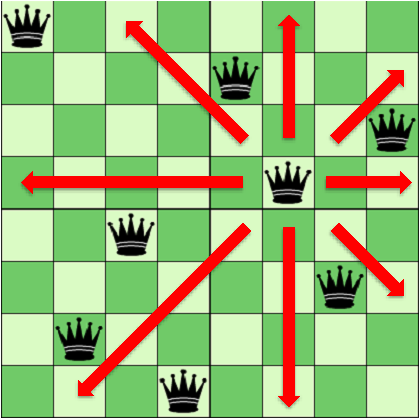
\includegraphics[height=100pt]{queen.png}
  \end{figure}
\end{frame}

\begin{frame}[fragile]{例题:八皇后问题}
  \begin{itemize}
    \item 枚举每个格子里是否有皇后,然后判断是否有冲突。\pause
    \item 复杂度 $O(2^{64})$ 原地爆炸\pause
    \item 枚举每行皇后的位置,然后判断是否有冲突。\pause
    \item 复杂度 $O(8^8)$,依旧有优化的空间
  \end{itemize}
\end{frame}

\begin{frame}[fragile]{例题:八皇后问题}
  \begin{itemize}
    \item 考虑在枚举每一个皇后的位置的时候同时检测是否有冲突,避免无用的搜索。\pause
    \item 具体可以利用数组 \verb|a[i][j]| 表示位置为 $(i,j)$ 的格子是否会被已经存在的皇后吃掉。\pause
    \item 每当放置一个皇后的时候,都需要更新可能会被该皇后吃掉的格子的 \verb|a[i][j]| 的值。\pause
    \item 当回溯的时候,可以恢复 \verb|a[i][j]| 的值。
  \end{itemize}
\end{frame}

\begin{frame}[fragile]{例题:八皇后问题}
  \begin{itemize}
    \item 具体为了简便更新和恢复 \verb|a[i][j]| 的值,每当我们放置皇后的时候就将影响到的格子的 \verb|a[i][j]| 的值加一,每当回溯的时候就将 \verb|a[i][j]| 的值减一。\pause
    \item 这样当且仅当 \verb|a[i][j]| $ = 0$ 时,该位置的格子才有可能被放置下一个皇后,否则就不再枚举该格子是皇后的可能性。
  \end{itemize}
\end{frame}

\begin{frame}[fragile]{例题:八皇后问题}
  \begin{minted}{cpp}
int a[8][8], ans = 0;
void effect(int x, int y, int delta) {
  for (int i = 0; i < 8; ++ i)
    for (int j = 0; j < 8; ++ j)
      if (i == x || j == y || abs(i - x) == abs(j - y))
        a[i][j] += delta;
}
void apply_queen(int x, int y) { effect(x, y, 1); }
void recover_queen(int x, int y) { effect(x, y, -1); }
  \end{minted}
\end{frame}

\begin{frame}[fragile]{例题:八皇后问题}
  \begin{minted}{cpp}
void dfs(int n) {
  // 如果已经放置了八个皇后,则输出结果
  if (n == 8) { ++ ans; return; }
  for (int i = 0; i < 8; ++ i) {
    for (int j = 0; j < 8; ++ j) {
      if (a[i][j] == 0) {
        apply_queen(i, j); // 放置皇后
        dfs(n + 1);
        recover_queen(i, j); // 回溯
      }
    }
  }
}
  \end{minted}
\end{frame}

\begin{frame}[fragile]{例题:八皇后问题}
  \begin{minted}{cpp}
int main() {
  dfs(0);
  std::cout << ans << std::endl;
  // 输出结果:3709440
}
  \end{minted}
  \pause
  可是答案不是 $92$ 么\pause

  显然我们枚举的时候没有考虑每个皇后的先后顺序,导致 $92$ 种不同的解都会被统计 $8!$ 次,因此答案为 $92 \times 8! = 3709440$
\end{frame}

\begin{frame}[fragile]{例题:八皇后问题}
  为了避免这种问题,我们可以在 dfs 的时候顺便带入一个 $(x, y)$ 坐标表示当前最后放置的皇后的位置,之后的枚举仅从这个位置的下一个格子开始。\pause

  稍微简化一点,第 $n$ 个皇后的位置必定在第 $n$ 行,因此我们在 DFS 中只需要枚举一行即可。
\end{frame}

\begin{frame}[fragile]{例题:八皇后问题(优化)}
  \begin{minted}{cpp}
void dfs(int n) {
  if (n == 8) { ++ ans; return; }
  for (int i = 0; i < 8; ++ i) {
    if (a[n][i] == 0) {
      apply_queen(n, i);
      dfs(n + 1);
      recover_queen(n, i);
    }
  }
} // dfs(0); std::cout << ans << std::endl; // 92
  \end{minted}
  \pause
  还能再快一点么
\end{frame}

\begin{frame}[fragile]{例题:八皇后问题(优化)}
  \begin{itemize}
    \item 考虑优化 \verb|apply_queen| 和 \verb|recover_queen| 的过程。
    \item 观察到总共只有 $64$ 个格子,每个格子我们只关心他的 0/1 状态。
    \item 因此我们可以把每个状态压缩到一个 \verb|unsigned long long| 里面。
    \item 预处理每个格子放置皇后会产生冲突的格子,转移的时候只需要将当前状态或上该转移状态即可。
  \end{itemize}
\end{frame}

\begin{frame}[fragile]{例题:八皇后问题}
  \begin{minted}{cpp}
uint64_t t[64]; // 转移状态
void init() {
  for (int x = 0; x < 8; ++ x)
    for (int y = 0; y < 8; ++ y)
      for (int i = 0; i < 8; ++ i)
        for (int j = 0; j < 8; ++ j)
          if (i == x || j == y || abs(i - x) == abs(j - y))
            t[(x << 3) | y] |= 1ull << ((i << 3) | j);
}
// O(n^4),当然也可以直接打表
  \end{minted}
\end{frame}

\begin{frame}[fragile]{例题:八皇后问题}
  \begin{minted}{cpp}
int ans = 0;
void dfs(int n, uint64_t state) {
  if (n == 8) { ++ ans; return; }
  for (int i = 0; i < 8; ++ i) {
    if (state & (1ull << ((n << 3) | i))) continue;
    dfs(n + 1, state | t[(n << 3) | i]);
  }
}
// dfs(0, 0); printf("%d\n", ans); // 92
  \end{minted}
\end{frame}

\begin{frame}[fragile]{剪枝优化}
  剪枝(Decision Tree Pruning, 决策树剪枝)是指在保证\textbf{正确性}的前提下,采取的一些手段使算法跳过一定不含有目标状态/最优解的分支,从而保证算法更高效迅速地找出目标解的状态。\pause

  一般的入手点有:

  \begin{itemize}
    \item \textbf{优化搜索顺序}:优先从比较优的转移状态开始搜索
    \item \textbf{可行性剪枝}:当前状态不含有目标状态,则直接跳过该状态的所有转移
    \item \textbf{最优性剪枝}:当前状态不含有更优解,则直接跳过该状态的所有转移
    \item \textbf{记忆化搜索}:对于一些纯函数的搜索,可以将搜索过的状态记录下来,避免重复搜索
  \end{itemize}
\end{frame}

\begin{frame}[fragile]{例题:[BeiJing2011]符环}
  给出一个长度为 $n(1 \le n \le 50)$ 的字符串 $S$,字符串仅包含 \verb|'S'| 和 \verb|'D'| 两种字母。

  询问有多少组合法的长度为 $2n$ 的括号序列 $R$ 满足:$(0 \le i < n)$

  \begin{itemize}
    \item 若 $S_i$ 为 \verb|'S'|,则 $R_i = R_{i+n}$
    \item 若 $S_i$ 为 \verb|'D'|,则 $R_i \ne R_{i+n}$
  \end{itemize}

  例如 $S$ 为 \verb|"SSD"|,则满足条件的 $R$ 有且仅有一种可能的解为 \verb|"()(())"|。\pause

  提示:枚举每一个 $R_i$,然后检查 $R$ 是否满足条件,复杂度为 $O(2^n \cdot n)$,考虑如何优化。
\end{frame}

\begin{frame}[fragile]{例题:[BeiJing2011]符环}
  DFS 的时候记录 $4$ 个状态,分别为:

  \begin{itemize}
    \item 当前搜索到的深度 $d$ 的位置
    \item 当前 $R[0:n]$ 中剩余未匹配的左括号数量
    \item 当前 $R[n:2n]$ 中左侧未匹配的右括号数量
    \item 当前 $R[n:2n]$ 中右侧未匹配的左括号数量
  \end{itemize}

  \begin{verbatim}
0      n-1 | n         2n-1
..(((..... | )))..(((......
  ^^^--- x | ^^^--- y
           |      ^^^--- z
  \end{verbatim}
\end{frame}

\begin{frame}[fragile]{例题:[BeiJing2011]符环}
  终止条件即为 $d = n$,同时我们返回当前的状态是否是一个合法的状态。

  \begin{minted}{cpp}
int dfs(int d, int x, int y, int z) {
  if (d == n) {
    return x == y && !z;
  }
  int ans = 0;
  \end{minted}

  接下来我们分情况讨论 $S_i$ 的类型。
\end{frame}

\begin{frame}[fragile]{例题:[BeiJing2011]符环}
  \begin{minted}{cpp}
  if (S[d] == 'S') {
    // put '('
    ans += dfs(d + 1, x + 1, y, z + 1);
    // put ')'
    if (x) {
      if (z) {
        ans += dfs(d + 1, x - 1, y, z - 1);
      } else {
        ans += dfs(d + 1, x - 1, y + 1, z);
      }
    }
  }
  \end{minted}
\end{frame}

\begin{frame}[fragile]{例题:[BeiJing2011]符环}
  \begin{minted}{cpp}
  if (S[d] == 'D') {
    // put '('
    if (z) {
      ans += dfs(d + 1, x + 1, y, z - 1);
    } else {
      ans += dfs(d + 1, x + 1, y + 1, z);
    }
    // put ')'
    if (x) {
      ans += dfs(d + 1, x - 1, y, z + 1);
    }
  }
  \end{minted}
\end{frame}

\begin{frame}[fragile]{复杂度分析}
  \begin{itemize}
    \item 首先复杂度十分玄学,不好直接利用公式量化计算。
    \item 但是我们可以通过观察,发现该算法相当于枚举了答案序列中的每一位。
    \item 因此该算法的复杂度是 $O(2^n)$,还能如何优化呢?
  \end{itemize}
\end{frame}

\begin{frame}[fragile]{复杂度分析}
  \begin{itemize}
    \item 观察发现 \verb|dfs(d, x, y, z)| 的返回值只与四元组 $(d, x, y, z)$ 有关,满足纯函数的定义。
    \item 而四元组 $(d, x, y, z)$ 可能的取值只有 $n^4$ 的情况。
    \item 因此利用记忆化搜索,该算法的复杂度可以降低到 $O(n^4)$。
  \end{itemize}
\end{frame}

\begin{frame}[fragile]{例题:[BeiJing2011]符环}
  \begin{minted}{cpp}
int f[52][52][52][52];
void init() { // 初始化记忆化缓存
  memset(f, -1, sizeof(f));
}
int dfs(int d, int x, int y, int z) {
  if (d == n) return x == y && !z;
  int &ans = f[d][x][y][z];
  if (~ ans) return ans;
  ans = 0;
  // 下略
}
  \end{minted}
\end{frame}

\section[广度优先搜索]{Breadth First Search}

\begin{frame}[fragile]{广度优先搜索}
  \begin{itemize}
    \item 就是每次都尝试访问同一层的节点
    \item 如果同一层都访问完了,再访问下一层
  \end{itemize}
\end{frame}

\begin{frame}[fragile]{例题:走迷宫}
  给出一张 $n \times m$ 的地图,其中 \verb|'#'| 表示墙,\verb|'.'| 表示可以走的路,\verb|'S'| 表示起点,\verb|'E'| 表示终点。

  请求出走迷宫的最短路径。

  \begin{verbatim}
##########
#S.......#
########.#
#T.......#
##########
  \end{verbatim}
\end{frame}

\begin{frame}[fragile]{例题:走迷宫}
  \begin{minted}{cpp}
int maze[52][52], dx = {0, 0, 1, -1}, dy = {1, -1, 0, 0};
int dfs(int x, int y) {
  if (x == tx && y == ty) return 0;
  int ans = INT_MAX;
  for (int i = 0; i < 4; ++i) {
    int nx = x + dx[i], ny = y + dy[i];
    if (inside_maze(nx, ny) && maze[nx][ny] != '#') {
      ans = min(ans, dfs(nx, ny) + 1);
    }
  }
  return ans;
}
  \end{minted}
\end{frame}

\begin{frame}[fragile]{例题:走迷宫}
  前面的 DFS 算法虽然可以解决一小部分的数据,但是如果遇到一些极端情况,则会导致复杂度暴增,甚至发生无限递归循环。

  这时候就应该需要使用广度优先搜索,每次一层一层的访问,直到找到终点。
\end{frame}


\begin{frame}[fragile]{广度优先搜索}
  广度优先搜索算法一般遵从以下几个步骤:
  
  \begin{itemize}
    \item 初始化一个队列,将起点或初始状态放入队列中
    \item 每次从队列中取出队首的状态,并对其进行处理
    \item 如果该状态是目标状态,则结束搜索
    \item 否则将该状态的所有后继未访问状态放入队列中
    \item 如果直到队列未空也没有找到目标状态,则说明无解
  \end{itemize}
\end{frame}

\begin{frame}[fragile]{例题:走迷宫}
  \begin{minted}{cpp}
char maze[52][52]; // 储存迷宫地图
int dis[52][52]; // 记录每个点到起点的距离
int dx = {0, 0, 1,-1}; // 四个方向的 delta x
int dy = {1,-1, 0, 0}; // 四个方向的 delta y
std::queue<std::pair<int, int>> q;
void bfs() {
  // 初始化起点
  q.push(std::make_pair(sx, sy));
  memset(dis, -1, sizeof(dis));
  dis[sx][sy] = 0;
  // 见下页
}
  \end{minted}
\end{frame}

\begin{frame}[fragile]{例题:走迷宫}
  \begin{minted}[fontsize=\small]{cpp}
while (!q.empty()) {
  int x = q.front().first, y = q.front().second;
  q.pop(); // 取出队首元素
  if (x == tx && y == ty) return dis[x][y];
  for (int i = 0; i < 4; ++ i) { // 枚举每一个方向
    int nx = x + dx[i], ny = y + dy[i];
    if (inside_maze(nx, ny) && maze[nx][ny] != '#'
        && dis[nx][ny] == -1) {
      dis[nx][ny] = dis[x][y] + 1;
      q.push(make_pair(nx, ny));
    }
  }
}
  \end{minted}
\end{frame}

\begin{frame}[fragile]{例题:中山市选[2009]小明的游戏}
  有一张 $n \times m$ 的地图,地图的格子分为 \verb|'@'| 和 \verb|'#'| 两种。

  每次从一个格子到达相邻的同类型格子,费用为 $0$,不同类型格子之间的费用则为 $1$。

  请求出小明从一个起点 $S$ 开始到达终点 $T$ 的最小费用。
\end{frame}

\begin{frame}[fragile]{例题:中山市选[2009]小明的游戏}
  非常经典的一道 BFS 题目,但是我们可以用一些巧妙的优化来加快搜索的速度。\pause

  在搜索的过程中,我们可以通过把队列中的每一个节点按照当前的距离排序,以此优化搜索顺序。
\end{frame}

\begin{frame}[fragile]{例题:中山市选[2009]小明的游戏}
  简单分析,发现我们并不需要每次都对当前队列中的所有元素进行枚举来找出距离最小的元素

  我们可以直接使用一种称为\textbf{堆}的数据结构来实现插入和询问最小值的操作。

  \begin{minted}{cpp}
typedef std::pair<int, int> Node; // 节点坐标
typedef std::pair<int, Node> DisNode; // 距离 + 坐标
// 小根堆
std::priority_queue<DisNode,
  std::vector<DisNode>,
  std::greater<DisNode>> q;
  \end{minted}
\end{frame}

\begin{frame}[fragile]{例题:中山市选[2009]小明的游戏}
  \begin{minted}[fontsize=\small]{cpp}
while (!q.empty()) {
  int d = q.top().first; // 当前距离
  int x = q.top().second.first, y = q.top().second.second;
  q.pop(); // 取出队首元素
  if (x == tx && y == ty) return d;
  for (int i = 0; i < 4; ++ i) { // 枚举每一个方向
    int nx = x + dx[i], ny = y + dy[i];
    if (nx >= 0 && nx < n && ny >= 0 && ny < m && !vis[nx][ny]) {
      vis[nx][ny] = 1;
      q.push(std::make_pair(d + (map[nx][ny] != map[x][y]),
                            std::make_pair(nx, ny)));
    }
  }
}
  \end{minted}
\end{frame}

\begin{frame}[fragile]{例题:中山市选[2009]小明的游戏}
  再深入分析一下,发现我们根本不需要使用堆来维护队列中的最小值。

  每次新加入的点的权值只有可能是当前队列中最小值加一或者相等,因此只需要考虑添加到队尾或者队首即可。

  \begin{minted}{cpp}
typedef std::pair<int, int> Node; // 节点坐标
std::deque<Node> q; // 双端队列
int dis[N][M]; // 距离
memset(dis, -1, sizeof(dis)); // 初始化
dis[sx][sy] = 0;
  \end{minted}
\end{frame}

\begin{frame}[fragile]{例题:中山市选[2009]小明的游戏}
  \begin{minted}[fontsize=\small]{cpp}
while (!q.empty()) {
  int x = q.front().first, y = q.front().second;
  q.pop_front(); // 取出队首元素
  if (x == tx && y == ty) return dis[x][y];
  for (int i = 0; i < 4; ++ i) { // 枚举每一个方向
    int nx = x + dx[i], ny = y + dy[i];
    if (nx >= 0 && nx < n && ny >= 0 && ny < m
        && dis[nx][ny] == -1) {
      dis[nx][ny] = dis[x][y] + (map[nx][ny] != map[x][y]);
      if (map[nx][ny] == map[x][y])
        q.push_front(std::make_pair(nx, ny));
      else q.push_back(std::make_pair(nx, ny));
    }
  }
}
  \end{minted}
\end{frame}

\begin{frame}[fragile]{例题:中山市选[2009]小明的游戏}
  以上使用\textit{双端队列}来优化 BFS 搜索的方式我们称之为 \textbf{0-1 BFS},经常被用于权值为 $0$ 或 $1$ 的图。
\end{frame}

\section[比较有意思的例题]{Examples}

\begin{frame}[fragile]{例题:水叮当的舞步}
  有一个 $n \times n$ 的地图,每个格子上有一种颜色 $c_{i,j}$,每次可以将地图左上角的格子和与其相连的所有相同颜色的格子都染成另一种颜色。

  问最少需要多少次染色才能将地图染成一种颜色?

  \begin{verbatim}
0 1 2
1 1 2
2 2 1
  \end{verbatim}

\end{frame}

\begin{frame}[fragile]{例题:水叮当的舞步}
  直接 DFS 搜索每次染成那种颜色,然后使用 BFS/DFS 修改染色结果。

  可以用下面几种剪枝优化:

  \begin{itemize}
    \item 如果染色前后左上角颜色的连通块大小不变,则直接剪枝
    \item 如果当前染色次数已经大于已经找到的最小染色次数,则直接剪枝
    \item 优先搜索染色后连通块大小最大的颜色,提高搜索效率
  \end{itemize}
\end{frame}

\begin{frame}[fragile]{例题:[Usaco2006 Jan] The Grove 树木}
  地图上有一个联通块(保证没有洞),贝茜在联通块外面的某一个点,可以往八个方向走,问贝茜至少需要走多少步才能绕林子走一圈,并且回到起点?

  \begin{verbatim}
.......   ...+...
...X...   ..+X+..
..XXX..   .+XXX+.
...XXX.   ..+XXX+
...X...   ..+X..+
......*   ...+++*
  \end{verbatim}
\end{frame}

\begin{frame}[fragile]{例题:[Usaco2006 Jan] The Grove 树木}
  可以从连通块中某一点往上画一条线,利用 BFS 算出每个点距离起点的距离,并且强行使得 BFS 枚举的时候不跨越这条线,最后统计一下这条线左右的距离合并即可。
\end{frame}

\begin{frame}[fragile]{例题:[SCOI2009]生日快乐}
  有一块大小为 $X \times Y$ 的蛋糕,现在需要将其平均分为 $N (N \le 10)$ 等分。每次只能平行于蛋糕的一边来切,显然必须要切 $N-1$ 刀。请求出这 $N$ 块蛋糕的长边与短边的比值的最大值的最小值。

  
\end{frame}

\begin{frame}[fragile]{例题:Whispers of the Old Gods}
  有一个正则表达式(只包含数字, \verb!|!, \verb|[|, \verb|]|, \verb|(|, \verb|)|, 和 \verb|+|)和一个数字串。

  每次可以对数字串进行一次操作,操作包括:

  \begin{itemize}
    \item 插入一个数字
    \item 删除一个数字
    \item 修改一个数字
  \end{itemize}

  请问至少需要多少次操作才能使得数字串匹配正则表达式?
\end{frame}

\begin{frame}[fragile]{例题:Whispers of the Old Gods}
  首先按照正则表达式构造出其对应的 NFA。

  之后在 NFA 上跑 0-1 BFS 即可。
\end{frame}

\begin{frame}[fragile]{汤普森构造法}

  汤普森构造法是一个能将正则表达式转化为一个与之等价的 NFA 的方法。算法得到的 NFA 可以在编程中用于匹配一个正则表达式,这也是正则表达式引擎实现的基本思路之一。

  从只包含一个字符的正则表达式看起,我们只需要将 $S$ 直接连一条匹配字符的边到 $T$ 即可。

  \begin{figure}[h]
    \centering
    \begin{tikzpicture}
      \node[circle,draw=black] (1) at(0,0) {$S$};
      \node[circle,draw=black] (2) at(4,0) {$T$};
      \draw[-latex] (1)--(2);
      \node at(2,0.5) {\verb|'a'|};
    \end{tikzpicture}
    \caption{匹配单个字符的 NFA}
  \end{figure}
\end{frame}

\begin{frame}[fragile]{汤普森构造法}
  对于 \verb!<regex> <regex>! 的顺序连接形式,我们只需要将第一个 NFA 的 $T$ 点连一条 $\varepsilon$ 边到第二个 NFA 的 $S$ 点即可。新的 NFA 的 $S$ 点即为 $S_1$,$T$ 点即为 $T_2$。

  \begin{figure}[h]
    \centering
    \begin{tikzpicture}
      \node[circle,draw=black] (1) at(2,0)  {$S_1$};
      \node[circle,draw=black] (2) at(4,0)  {$T_1$};
      \node[circle,draw=black] (3) at(8,0)  {$S_2$};
      \node[circle,draw=black] (4) at(10,0) {$T_2$};
      \draw[-latex] (2)--(3);
      \node at(6,0.5) {$\varepsilon$};
      \draw (3,0) ellipse (2 and 1);
      \draw (9,0) ellipse (2 and 1);
    \end{tikzpicture}
    \caption{顺序连接两个表达式的 NFA}
  \end{figure}
\end{frame}

\begin{frame}[fragile]{汤普森构造法}
  对于 \verb!<regex> | <regex>! 或者 \verb|[<atom-regex-list>]| 的逻辑或形式,我们需要新建两个节点 $S$ 和 $T$,然后从 $S$ 节点向各个 $S_i$ 节点连 $\varepsilon$ 边,从各个 $T_i$ 节点向 $T$ 节点连 $\varepsilon$ 边。$S$ 和 $T$ 即为新 NFA 的起始点和终止点。

  \begin{figure}[h]
    \centering
    \begin{tikzpicture}
      \node[circle,draw=black] (1) at(2,0) {$S_2$};
      \node[circle,draw=black] (2) at(4,0) {$T_2$};
      \node[circle,draw=black] (3) at(2,2) {$S_1$};
      \node[circle,draw=black] (4) at(4,2) {$T_1$};
      \node[circle,draw=black] (5) at(-1,1) {$S$};
      \node[circle,draw=black] (6) at(7,1) {$T$};
      \draw[-latex] (5)--(1);
      \draw[-latex] (5)--(3);
      \draw[-latex] (2)--(6);
      \draw[-latex] (4)--(6);
      \draw (3,0) ellipse (2 and 0.9);
      \draw (3,2) ellipse (2 and 0.9);
      \node at(0.5,0.8) {$\varepsilon$};
      \node at(0.5,1.8) {$\varepsilon$};
      \node at(5.5,0.8) {$\varepsilon$};
      \node at(5.5,1.8) {$\varepsilon$};
    \end{tikzpicture}
    \caption{匹配分支形式的 NFA}
  \end{figure}
\end{frame}

\begin{frame}[fragile]{汤普森构造法}
  对于出现一次或者多次的逻辑,即 \verb|<regex> +| 语法,我们可以直接连一条 $T$ 到 $S$ 的 $\varepsilon$ 边。

  \begin{figure}[h]
    \centering
    \begin{tikzpicture}
      \node[circle,draw=black] (1) at(2,0) {$S$};
      \node[circle,draw=black] (2) at(4,0) {$T$};
      \draw (3,0) ellipse (2 and 1);
      \draw[-latex] (4,0.4) arc (0:180:1);
      \node at(3,1.8) {$\varepsilon$};
    \end{tikzpicture}
    \caption{匹配一次或多次的 NFA}
  \end{figure}
\end{frame}

\begin{frame}[fragile]{汤普森构造法}
  对于出现零次或一次的逻辑,即 \verb|<regex> ?| 语法,我们可以通过类似分支形式的方式实现。

  \begin{figure}[h]
    \centering
    \begin{tikzpicture}
      \node[circle,draw=black] (1) at(2,0) {$S_1$};
      \node[circle,draw=black] (2) at(4,0) {$T_1$};
      \node[circle,draw=black] (3) at(0,0) {$S$};
      \node[circle,draw=black] (4) at(6,0) {$T$};
      \draw (3,0) ellipse (2 and 1);
      \draw[-latex] (3)--(1);
      \draw[-latex] (2)--(4);
      \draw[-latex] (0,0.4) arc (180:0:3 and 1);
      \node at(3,1.8) {$\varepsilon$};
    \end{tikzpicture}
    \caption{匹配零次或一次的 NFA}
  \end{figure}
\end{frame}

\begin{frame}[fragile]{例题:Whispers of the Old Gods}
  按照汤普森构造法构造出一个 NFA 之后,我们便可以在该 NFA 上进行 0-1 BFS 搜索。

  搜索的时候记录两个值,当前到达的节点 $X$ 和原串目前匹配到的位置 $p$,并将 $\{X, p\} (X \in V_{NFA}, 0 \le p \le n)$ 二元组看作新的节点。
\end{frame}

\begin{frame}[fragile]{例题:Whispers of the Old Gods}
  接下来考虑节点 $\{X, p\}$ 有那些转移:

  \begin{enumerate}
    \item \textbf{删除字符}:$\{X, p\}$ 可以花费 $1$ 代价转移到 $\{X, p+1\}$
    \item \textbf{匹配 $\varepsilon$ 边}:若存在 $\varepsilon$ 边 $X \to Y$,则$\{X, p\}$ 可以直接转移到 $\{Y, p\}$
    \item \textbf{匹配字符}:若存在字符 $a$ 边 $X \to Y$,且 $S_{p+1}=a$,则 $\{X, p\}$ 可以直接转移到 $\{Y, p+1\}$
    \item \textbf{修改字符}:若存在字符 $a$ 边 $X \to Y$,且 $S_{p+1} \ne a$,则 $\{X, p\}$ 可以花费 $1$ 代价转移到 $\{Y, p+1\}$
    \item \textbf{插入字符}:若存在字符 $a$ 边 $X \to Y$,则 $\{X, p\}$ 可以花费 $1$ 代价转移到 $\{Y, p\}$
  \end{enumerate}

  最终问题转化为求从 $\{S, 0\}$ 开始到 $\{T, n\}$ 的最短路问题,可以通过 0-1 BFS 算法解决。
\end{frame}

\begin{frame}{}
  \centering \Large
  \emph{Good Luck \& Have Fun!}
\end{frame}

\end{document}